\chapter{系统总体设计}\label{chap:systemoveral}

本章将介绍系统的总体设计结构,包括硬件验证平台的选择,系统的任务划分,加速器 与 ARM 互联的,对用户友好的演示页面的介绍等。

\section{用户友好的输入页面设计方案}

如图~\ref{fig:BootStrap}所示,本设计基于 Bootstrap 与 Flask 等 Web 应用技术开发了用户友好的输入页面与数据显示页面。

\begin{figure}[!htbp]
    \centering
    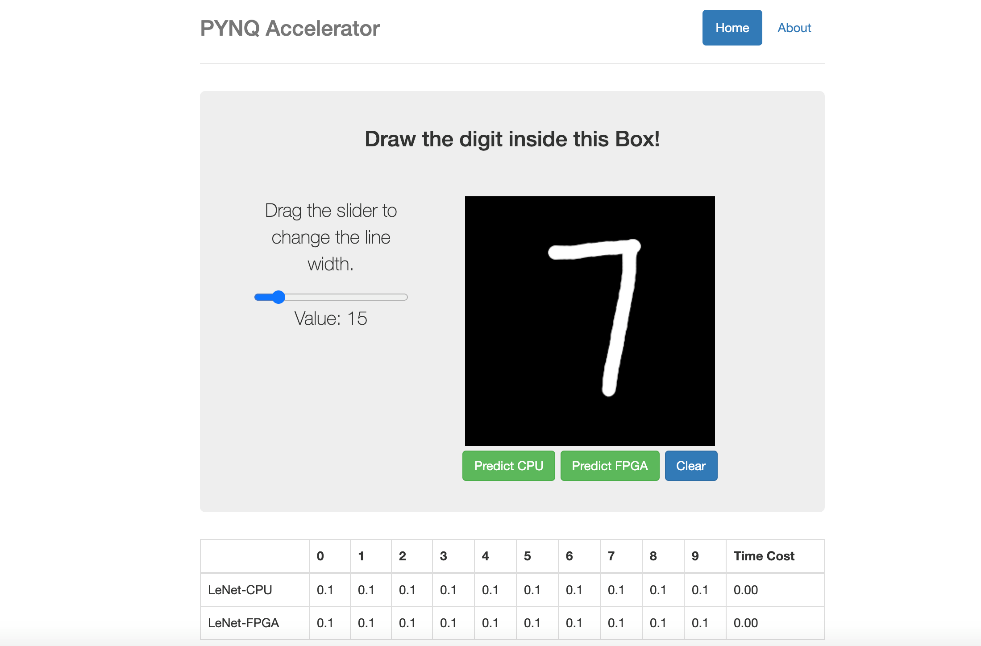
\includegraphics[width=0.7\textwidth]{bootstrap}
    \caption{用户友好的输入页面}
    \label{fig:BootStrap}
\end{figure}

Bootstrap 是由 Twitter 推出的用于前端开发的开源工具包,它简洁灵活,功能强大,本次设计初始阶段使用 Bootstrap 设计了一个手写数字页面,用户可以通过鼠标在 Canvas 画布上调节画笔大小,绘制数字,通过按键来决定采用 ARM 或者 FPGA 进行深度神经网络的推理。

当用户按下按键之后,Web 前端会使用 Ajax 发送 HTTP 请求,通过以太网与开发板通信,获取处理结果。在板卡上,本设计使用 Flask 部署了Web应用的后端,负责接受 HTTP 请求,决策推理平台,将推理结果以及相关信息打包发送 HTTP 响应。

\section{硬件设计架构与互联}

本设计的硬件总体架构设计如图~\ref{fig:Hardware System Connect}所示,深度神经网络专用的加速器体系应该作为通用处理器的一个协处理器而存在。本设计选取的主控制器为双核的 ARM A9。

\begin{figure}[!htbp]
    \centering
    \includegraphics[width=0.5\textwidth]{HardwareSystemConnect.pdf}
    \caption{硬件总体设计架构}
    \label{fig:Hardware System Connect}
\end{figure}

在设计的初期,加速器(Accelerator,ACC)参考了 CNNIOT 设计了通用的卷积神经网络加速器,其支持配置可以调节的卷积、池化、激活函数、全连接等基本卷积神经网络算子。基于该加速器,设计实现了手写数字识别网络 LeNet5,平均处理一张图像需要 168ms,而 Arm A9 处理一张图像需要 1204ms,为了实现整个网络,需要做的事情如下:

\begin{enumerate}
    \item 使用 Caffe 预训练模型得到 Caffemodel 文件。
    \item 使用 Netron 将 Caffemodel 文件内部的权重参数导出为二进制文件。
    \item 由加速器设计神经网络结构,并进行推理。
\end{enumerate}

针对仅有三层卷积层,两层全连接层的 Lenet5 网络来说,配置的过程已经十分复杂,更不用说设计包含残差结构的 Resnet 网络。由此可以看出,硬件加速器被设计出来只是第一步,还需要构建完整的软件栈体系。

在经过一番调研之后,加速器设计选择了英伟达公司开源的 NVDLA 框架,经过英伟达团队几年的努力,NVDLA 自上而下打通了软件栈与硬件栈,可以实现端到端的推理,是一个适合深入学习的框架。

在 Xilinx 的设计工具中提供的 IP 核大多使用 AXI4 总线来实现各级之间的逻辑控制和数据传输。前文中提到,NVDLA 亦是使用 AXI4 总线访问存储,无疑极大方便了我们的设计,但是 NVDLA 的控制总线协议不是 AXI4 协议,在本设计中,其通过 csb2apb 电路将 CSB 协议转换为 APB 总线协议,在 Vivado 设计中,我们使用 Xilinx 官方提供给的 APB2AXI Bridge IP 将 APB 总线再转换为 AXI4 总线挂载到 ARM 处理器上。

\section{验证平台}

NVDLA 加速器设计需要挂载到 Linux 内核上,所以本设计需要一款通用处理器作为主控,并且移植 Linux 操作系统。并且,考虑到本设计采用的 small 配置需要7万以上的查找表资源。则可供选型的器件型号有:

\begin{enumerate}
    \item ZYNQ 7000 系列,该芯片集成了一块双核32位 ARM A9 处理器作为主控制器,而 FPGA 侧的资源随芯片的型号不同而不同,想要实现 NVDLA 至少需要使用到 ZYNQ 7045 器件。
    \item ZYNQ MPSoc 系列,该芯片集成了一块多核的64位的 ARM A53 处理器作为主控制器,性能相较于 ZYNQ 7000 器件强,官方开发板卡的价格在2万左右。
    \item 纯FPGA逻辑器件,如官方板卡 VCU118,有足够大的LUT资源,可以将 RISC-V 处理器与 NVDLA 一起实现,并在 RISC-V 处理器上移植 Riscv-   RISC-V 处理器,开发周期较长。
\end{enumerate}

综合以上,本设计选用的器件型号为 XC7Z045-2FFG900I,开发板卡为如图~\ref{fig:ZYNQ 7045}的第三方板卡,价格为三千多元人民币。

\begin{figure}[!htbp]
    \centering
    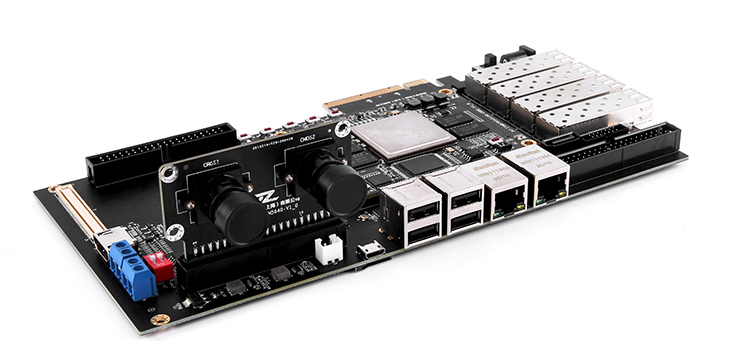
\includegraphics[width=0.9\textwidth]{ZYNQ 7045.jpeg}
    \caption{ZYNQ 7045 开发板}
    \label{fig:ZYNQ 7045}
\end{figure}


